\section{22.10.2014 - Termostatazione}

In questa esperienza costruiremo un termometro elettronico utilizzando una Pt100. Realizzeremo poi un sistema di controllo proporzionale di temperatura utilizzando il termometro da noi costruito. 

\subsection*{Strumenti e materiali}

\begin{figure}[htc]
\begin{itemize} [noitemsep]
	\item Generatore di forme d'onta Agilent 33120A con range di frequenza da \SI{100}{\micro\hertz} a \SI{15}{\mega\hertz};
	\item Oscilloscopio Agilent DSO-X 2002A (bandwidth \SI{70}{\mega\hertz}, sample rate \num{2} GSa/s);\newline
	\begin{minipage}{0.65\textwidth}
		\vspace{0.4mm}
%		\begin{itemize} [noitemsep]
%		\item Oscilloscopio Agilent DSO-X 2002A (bandwidth \SI{70}{\mega\hertz}, sample rate \num{2} GSa/s);
		\item Generatore di tensione continua Agilent E3631A (max $\pm \, \SI{25}{\volt}$ o $\pm \, \SI{6}{\volt}$);
%		\item Generatore di forme d'onta Agilent 33120A con range di frequenza da \SI{100}{\micro\hertz} a \SI{15}{\mega\hertz};
		\item Multimetro Agilent 34410A a sei cifre e mezza;
		\item Tre amplificatori operazionali OP07;
		\item Un integrato AD622 e un REF02;
		%\item Un integrato REF02;
		\item Una termoresistenza PT100;
		\item Transistor di potenza NPN 2N2222;
		\item Resistenze e capacità di vari valori;
		\item Trimmer multigiro da \SI{10}{\kilo\ohm} e \SI{1}{\kilo\ohm};
		\item Breadboard e cablaggi vari.
%		\end{itemize}
	\end{minipage}
	%\begin{minipage}{0.3\textwidth}
	%		\centering
	%		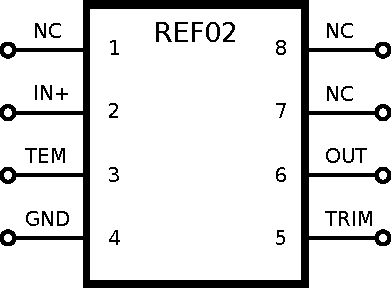
\includegraphics[width=3.5cm]{../E06/latex/REF02.pdf}
	%		\caption{Piedinatura dell'integrato\newline REF02.}
	%		\label{cir6:REF02}
%2 è alimentato con +\SI{15}{\volt}, 4 è collegato a comune, 6 restituisce una tensione costante di +\SI{5}{\volt}.}
	%\end{minipage}
\end{itemize}
\end{figure}
\vspace{-.8cm}


\subsection{Termometro elettronico}

%\begin{wrapfigure}[6]{r}{0.6\textwidth}
%\centering
%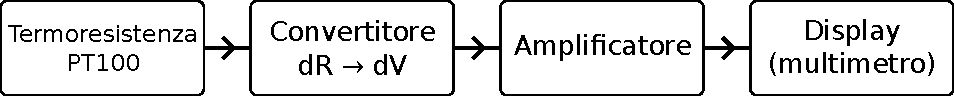
\includegraphics[width=.6\textwidth]{../E06/latex/s1.pdf}
%\caption{Schema logico del termometro elettronico.}
%\label{fig6:scheme1}
%\end{wrapfigure}

In questa prima parte vogliamo realizzare un termometro elettronico.
Per far ciò usiamo una termoresistenza Pt100 di resistenza 100\si{\ohm} a zero gradi Celsius.



Realizzeremo il nostro circuito blocchi, in modo da testarne il funzionamento singolarmente ed evitare pertanto di dover effettuare alla fine la ricerca di eventuali errori su tutto il circuito.
%Inoltre posizioneremo dei punti tra i blocchi appositamente per effettuare misure intermedie.

\subsubsection{Convertitore Resistenza-Tensione}
Per convertire la variazione di resistenza della Pt100 -- generata a sua volta da una variazione in temperatura della stessa -- in tensione, dobbiamo far scorrere in essa una corrente.
Per evitare surriscaldamenti abbiamo scelto una corrente di \SI{1}{\milli\ampere}.
%
%\subsubsection*{
\paragraph{Generatore di corrente costante [Blocco 1]\newline}

\begin{wrapfigure}[13]{r}{0.3\textwidth}
\centering
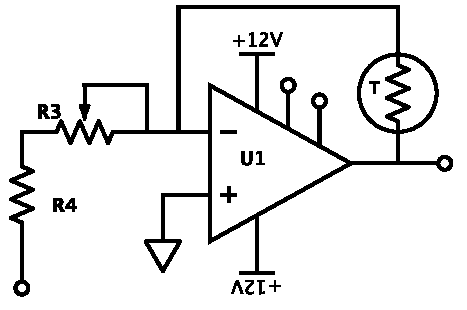
\includegraphics[width=.3\textwidth]{../E06/latex/P1.pdf}
\caption{Blocco 1: Generatore di corrente costante.}
\label{cir6:blocco1}
\end{wrapfigure}

Come primo blocco realizziamo un generatore di corrente costante.
Come sappiamo, la tensione che scorre nel ramo di retroazione è univocamente determinata dalla tensione all'ingresso invertente e dalla resistenza posta all'ingresso invertente.
Dobbiamo stare attenti che il nostro opamp non vada in saturazione o avremo una dipendenza della corrente dal carico.

Da una semplice analisi circuitale, otteniamo che $I=V_{in}/(\SI{4.7}{\kohm}+T_1)$.
È stato scelto di utilizzare come resistenza all'ingresso invertente un resistenza da \SI{4.7}{\kilo\ohm} con in serie un trimmer multigiro da \SI{1}{\kilo\ohm}.
Così facendo, utilizzando un amperometro in serie, possiamo tarare con precisione la corrente che scorre nel ramo di retroazione (e dunque nella nostra termoresistenza).
Durante questa fase non utilizzeremo la termoresistenza\footnote{non utilizzeremo la termoresistenza per evitare di rovinarla in quanto è un componente particolarmente costoso.}, ma una comune resistenza di valore nominale \SI{100}{\ohm}.

Con una corrente scelta di \SI{1}{\milli\ampere}, la potenza dissipata per effetto Joule dalla nostra termoresistenza è $P=I^2 R \cong \SI{.1}{\mW}$.
%
%STIMA DELL'ERRORE DATO DALL'AUTORISCALDAMENTO

%\subsubsection*{
\paragraph{Generatore di tensione costante\newline}

Per alimentare il blocco 1 con un segnale $V_{in}$ stabile, abbiamo scelto di usare l'integrato REF02.
Alimentandone il piedino 2 con +\SI{15}{\volt} e collegando il piedino 4 a comune, il piedino 6 restituisce una tensione costante di +\SI{5}{\volt} con un incertezza di \num{0.3}$\%$.
\newpage

\subsubsection{Amplificazione e Condizionamento del segnale}
Una volta convertito il segnale in tensione, vogliamo che esso scali con una $\Delta V=\SI{100}{\milli\volt}/\si{\celsius}$.
Inoltre vogliamo ottenere una lettura di tensione pari a \num{0} quando la temperatura ambientale è di \SI{0}{\celsius}.
Per fare ciò introduciamo in serie al blocco 1 due blocchi di alimentazione e di condizionamento.

%\subsubsection*{
\paragraph{Amplificazione [Blocco 2]\newline}

\begin{wrapfigure}[12]{r}{0.4\textwidth}
\centering
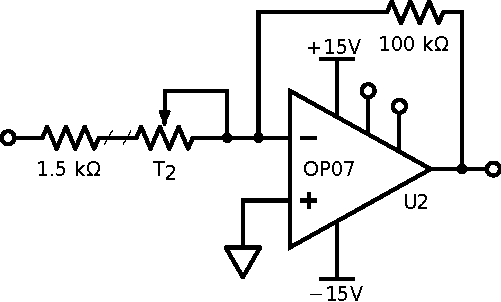
\includegraphics[width=.3\textwidth]{../E06/latex/P2.pdf}
\caption{Amplificatore con G=50.}
\label{cir6:blocco2}
\end{wrapfigure}

A \SI{0}{\celsius} la tensione in uscita al blocco 1 è di \SI{-100}{\mV} (il segno meno è dovuto alla configurazione invertente del blocco 1).
Come prima cosa amplifichiamo tale segnale in modo che (con \SI{0}{\celsius}) la tensione in uscita dal blocco 2 sia di \SI{5}{\volt}.
Così facendo, possiamo usare un comparatore con $V_{ref}=\SI{5}{\volt}$ che restituirà in uscita \SI{0}{\volt} per $T=\SI{0}{\celsius}$.

Per tarare il Gain del nostro amplificatore (che ovviamente dovrà essere G=\num{-50}), abbiamo deciso di utilizzare un segnale DC di \SI{-100}{\mV} dall'Agilent E3631A portato all'ingresso invertente (l'ingresso non invertente è stato collegato a comune).
Abbiamo utilizzato una resistenza di feedback di \SI{100}{\kilo\ohm} mentre la resistenza all'ingresso invertente è stata costruita mettendo in serie una resistenza nominale da \SI{1.5}{\kilo\ohm} e un trimmer multigiro da \SI{1}{\kilo\ohm}.
Così facendo è stato possibile tarare perfettamente il guadagno a \num{-50}, che evidentemente si ha quando la tensione in uscita è \SI{5}{\volt}. 

%\subsubsection*{
\paragraph{Condizionamento [Blocco 3]\newline}

\begin{wrapfigure}[13]{r}{0.4\textwidth}
\centering
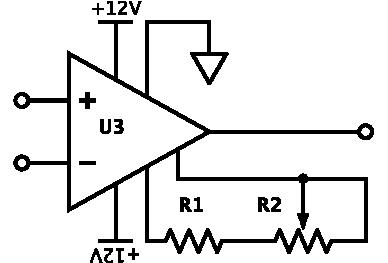
\includegraphics[width=.27\textwidth]{../E06/latex/P3.pdf}
\caption{Amplificatore differenziale con G=5.195.}
\label{cir6:blocco3}
\end{wrapfigure}

Portando ora il segnale amplificato in uscita dal blocco 2 all'ingresso non invertente di un amplificatore per strumentazione (AD622) e utilizzando come riferimento i \SI{5}{\volt} forniti dal generatore di tensione REF02 si ottiene facilmente che, quando la temperatura dell'ambiente è di \SI{0}{\celsius}, l'AD622 avrà un'uscita nulla.
Quando la temperatura è maggiore di zero anche l'uscita del blocco 3 sarà maggiore di zero, perchè la tensione all'ingresso non invertente (segnale della temperatura) è maggiore del riferimento ($5\si{\volt}$).

Dobbiamo ora decidere il guadagno dell'AD622.
Per far ciò basta ricordare che vogliamo ottenere è un $\Delta V=\SI{100}{\milli\volt}/\si{\celsius}$, così da avere una conversione in gradi centigradi a meno di un fattore 10.
Poiché il blocco 1 resistuisce una variazione per ogni grado centigrado di $\Delta V=\SI{0.385}{\milli\volt}/\si{\celsius}$, il guadagno totale dev'essere di
$$G\,=\,\frac{\SI{100}{\milli\volt}/\si{\celsius}}{\SI{0.385}{\milli\volt}/\si{\celsius}}=\num{259.740}$$
(il segno meno è dato ancora una volta dalla configurazione invertente del blocco 1).
Il guadagno totale è però determinato separatamente da U2 e U3 e deve valere $G= G_{U2}\cdot G_{U3}=-259.740$ .
È dunque immediato verificare che imponendo $G_{U2}=-50$ deve valere $G_{U3}=5.195$.


\begin{figure}[ht]
 \centering
   {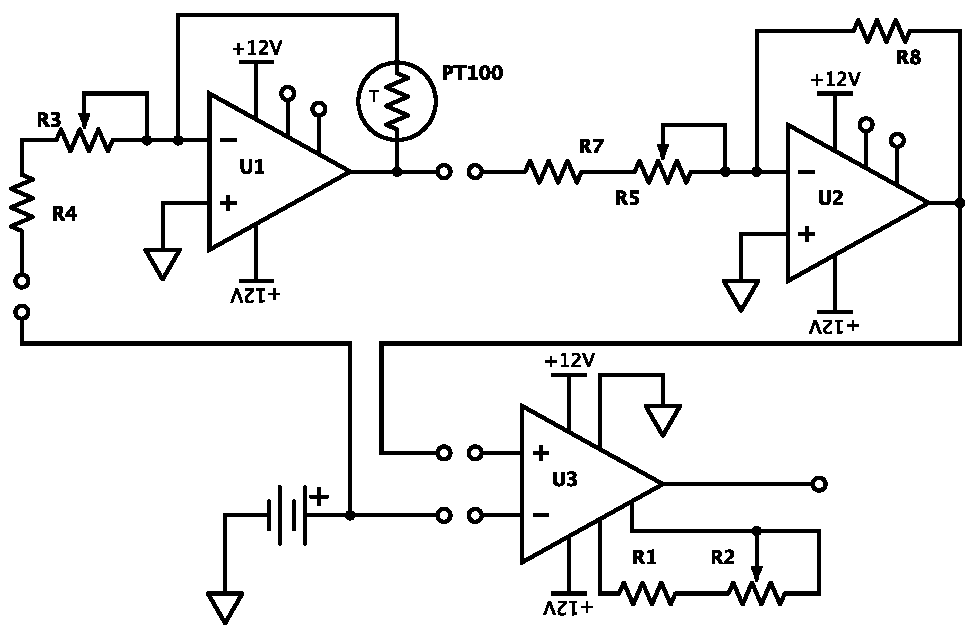
\includegraphics[width=0.7\textwidth]{../E06/latex/c1.pdf}}
 \caption{Schema circuitale del termometro elettronico.}
 \label{cir6:term}
\end{figure}


\vspace{-2mm}
\subsection{Sistema di controllo proporzionale}

\begin{wrapfigure}[12]{r}{0.5\textwidth}
\centering
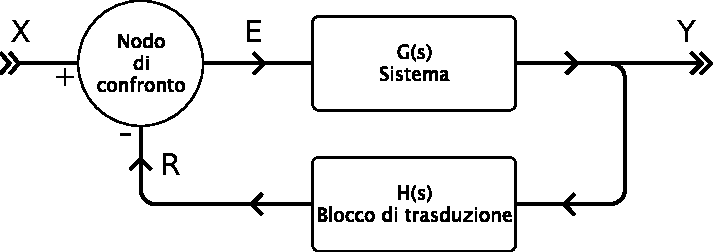
\includegraphics[width=.5\textwidth]{../E06/latex/s2.pdf}
\caption{Schema logico del sistema di controllo proporzionale di temperatura.}
\label{fig6:scheme2}
\end{wrapfigure}

Aggiungiamo ora al circuito proposto nel paragrafo precedente un sistema di controllo proporzionale, la cui funzione sarà quella di riscaldare una resistenza fino a raggiungere una data temperatura di soglia.

Per comprenderne meglio l'implementazione, generalizziamo prima il concetto di controllo proporzionale.
Osserviamo lo schema in Figura \ref{fig6:scheme2}: dati due segnali in ingresso X e R , il sistema deve rispondere con Y  se viene rispettata una condizione controllata dal nodo di confronto.
Quest'ultimo avrà dunque il compito di confrontare X ed R e verificare che la condizione, in generale funzione dei due segnali, sia rispettata.
L'aggiornamento di tale condizione è invece affidato al blocco di retroazione, che varia R.

Nel nostro caso, X è la tensione relativa alla temperatura di soglia ($T_{S}$) e R la tensione relativa alla temperatura misurata dalla termoresistenza ($T$).
La nostra Y sarà una data potenza dissipata su una resistenza di potenza che, se posta vicino alla PT100, ne varierà il valore di resistenza e quindi la temperatura letta dal circuito.
Dobbiamo ora identificare i blocchi relativi al sistema di controllo proporzionale e progettare quelli mancanti al circuito attuale.

Affidiamo il compito del blocco di retroazione al circuito finora costruito: questo restituisce un valore di tensione proporzionale alla temperatura letta dalla termoresistenza, che dovrà essere confrontato con la soglia.
Successivamente, il blocco di controllo deve fare la differenza fra questi due valori e, una volta raggiunto un valore impostabile, diminuire il valore della corrente fornita alla resistenza di potenza in maniera proporzionale ad E.
Definiamo dunque E=X-R, e per effettuare tale operazione utilizziamo un amplificatore differenziale.
Infine, per fornire la corrente necessaria alla resistenza, utilizzeremo un transistor BJT di potenza.
\vspace{-2mm}
\subsubsection{Confronto [Blocco 4]}

\begin{wrapfigure}[13]{r}{0.37\textwidth}
\centering
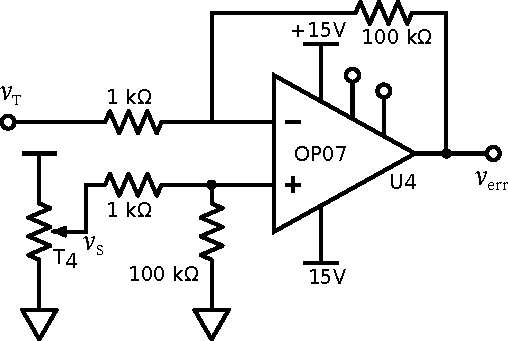
\includegraphics[width=.33\textwidth]{../E06/latex/P4.pdf}
\caption{Blocco di confronto}
\label{fig6:blocco4}
\end{wrapfigure}

Analizziamo il blocco di confronto proposto in Figura \ref{fig6:blocco4}.
Con il trimmer impostiamo una tensione $V_{S}$ proporzionale a $T_{S}$ (bisogna rispettare l'output del circuito precedente per impostarla, cioè $T_S = \frac{V_S}{\SI{100}{\milli\volt\per\celsius}}$) che può essere confrontata direttamente con la tensione $V_{T}$ relativa a $T$ in arrivo dal blocco di retroazione.
Inoltre, ponendo le resistenze uguali a \SI{1}{\kilo\ohm} e \SI{100}{\kilo\ohm} nel circuito di retroazione dell'amplificatore come in Figura, otteniamo un guadagno $G=100$.

Definendo la tensione in uscita dall'operazionale come $V_{err}$ e
$$\Delta T = \frac{|V_{S}-V_{T}|}{\SI{100}{\milli\volt}/\si{\celsius}}= | T_S - T | $$
Ovviamente, per valori di tensione in entrata maggiori di $\approx \SI{.15}{\volt}$, l'opamp entrerà in saturazione, mandando $V_{err}\approx \SI{15}{\volt}$; altrimenti l'amplificazione sarà quella di un amplificatore invertente.
Dunque varrà la seguente equazione (per $\Delta V = |V_S - V_T|$)

\begin{equation}
V_{err} = \bigg \{
\begin{array}{rl}
G \,\Delta V = G \,\Delta T \,\SI{100}{\milli\volt}/\si{\celsius}  & \mathrm{se} \quad 0<\Delta V<0.15 \si{\volt} \\
V_{U4}^{sat}\approx 15 \si{\volt} & \mathrm{se} \quad \Delta V>0.15 \si{\volt} \\
\end{array}
\label{eq6:exit_opamp}
\end{equation}

\subsubsection{Sistema [Blocco 5]}

\begin{wrapfigure}[17]{r}{0.2\textwidth}
\centering
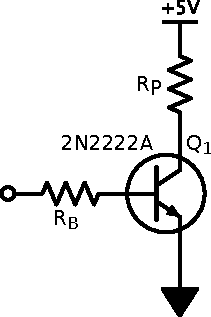
\includegraphics[height=3.5cm]{../E06/latex/P5.pdf}
\caption{Sistema di riscaldamento proporzionale}
\label{fig6:sistema}
\end{wrapfigure}

Per progettare il sistema di riscaldamento proporzionale, dobbiamo fornire potenza (ad una resistenza capace di dissipare molta energia e quindi di sopportare alti valori di corrente, detta \textit{resistenza di potenza}) in maniera proporzionale ad E, cioè $\Delta T$.
Per fare ciò, utilizzeremo un transistor 2N2222A con emettitore collegato a comune, le cui caratteristiche sono le seguenti
%$$\begin{array}{rl}
%\beta = \frac{I_c}{I_b} = 75\\
%V_{CE}^{sat}=0.4 \si{\volt}\\
%V_{BE}^{pol}=1.3 \si{\volt}\\
%\end{array}$$
$$\beta=\frac{I_c}{I_b}=75 \qquad V_{CE}^{sat}=\SI{.4}{\volt} \qquad V_{BE}^{pol}=\SI{1.3}{\volt}$$
Vale che, con una resistenza di potenza $R_{P} = \SI{27}{\ohm}$ e impostata una tensione di $5$ \si{\volt} costante ad uno dei suoi capi\footnote{Il REF02 non avrebbe potuto erogare la corrente necessaria a mantenere invariata la tensione ai capi della resistenza.
Dunque, per gestire questa tensione, abbiamo utilizzato il generatore di tensione costante Agilent E3631A.
Inoltre, per questo motivo, la comune utilizzata per questo blocco è stata posta indipendentemente per poi essere collegata a quella degli altri blocchi.} come in Figura \ref{gr6:proporzionale},
$$I_{C}=\frac{5 \si{\volt}- V_{CE}^{sat}}{R_P}=170 \si{\milli\ampere}$$
quindi $I_B=I_{C}/\beta=\SI{2.27}{\mA}$, da cui otteniamo il valore per cui il transistor si trova in saturazione (cioè quando la tensione base emettitore è pari a $V_{BE}^{pol}$ e la tensione base collettore è uguale a $V_{CE}^{sat}$)
$$R_B=\frac{V_{err} - V_{BE}^{pol}}{I_B}=2.2 \si{\kilo\ohm}$$

Considerando il seguente sistema che descrive il transistor e le resistenze calcolate in precedenza
$$
\begin{cases}
\begin{array}{rl}
\SI{5}{\volt}-V_{CE}^{sat} \geq \SI{5}{\volt}-V_{CE} = I_{C}R_P\\
I_C=\beta I_B \\
V_B - V_E = V_{BE} \leq V_{BE}^{pol} = V_{BE}^{sat}\\
V_{err}-V_B=I_B R_B
\end{array}
\end{cases}
$$
si può ottenere la condizione di saturazione come una condizione su $V_{err}$
\begin{equation}
V_{err}^{sat} \geq \frac{5\si{\volt}-V_{CE}^{sat}}{\beta} \frac{R_B}{R_P}+V_{BE}^{sat} \cong 6.3 \si{\volt}
\label{eq6:saturazione}
\end{equation}
e una condizione di interdizione (data da $I_C = 0 \Rightarrow I_B = I_C / \beta = 0$)
\begin{equation}
V_{err}^{int} = I_B R_B + V_B = V_B \leq V_{BE}^{pol} = \SI{1.3}{\V}
\label{eq6:interdizione}
\end{equation}
Per tensioni superiori a $V_{err}^{sat}$ il transistor sarà in zona di saturazione, per tensioni inferiori a $V_{err}^{int}$ sarà in interdizione e nella regione intermedia esso sarà governato linearmente dalla corrente di base.

Dunque, date (\ref{eq6:exit_opamp}), (\ref{eq6:saturazione}) e (\ref{eq6:interdizione}), il massimo della corrente e quindi, per la legge di Joule, il massimo della potenza dissipata da $R_P$ si avrà per $\Delta T \gtrsim 0.63 \si{\celsius}$), mentre il nostro circuito disabiliterà l'alimentazione della resistenza interdicendo il transistor per $\Delta V \lesssim \SI{.13}{\V}$, cioè quando la temperatura ambientale si porterà entro $\approx \SI{0.13}{\celsius}$ da $T_{S}$.


Ad un siffatto sistema abbiamo inoltre aggiunto un LED in modo tale che fosse acceso quando la resistenza $R_P$ fosse alimentata e fosse spendo quando il transistor fosse interdetto.
Per raggiungere tale scopo il diodo è stato messo in serie ad una resistenza da \SI{500}{\ohm} su un ramo parallelo alla resistenza di potenza $R_P$ affinché vi scorresse una corrente di circa \SI{10}{\mA}.
Tale particolare si può osservare nello schema circuitale in Figura \ref{gr6:proporzionale}.



\begin{figure}[htc!]
 \centering
   {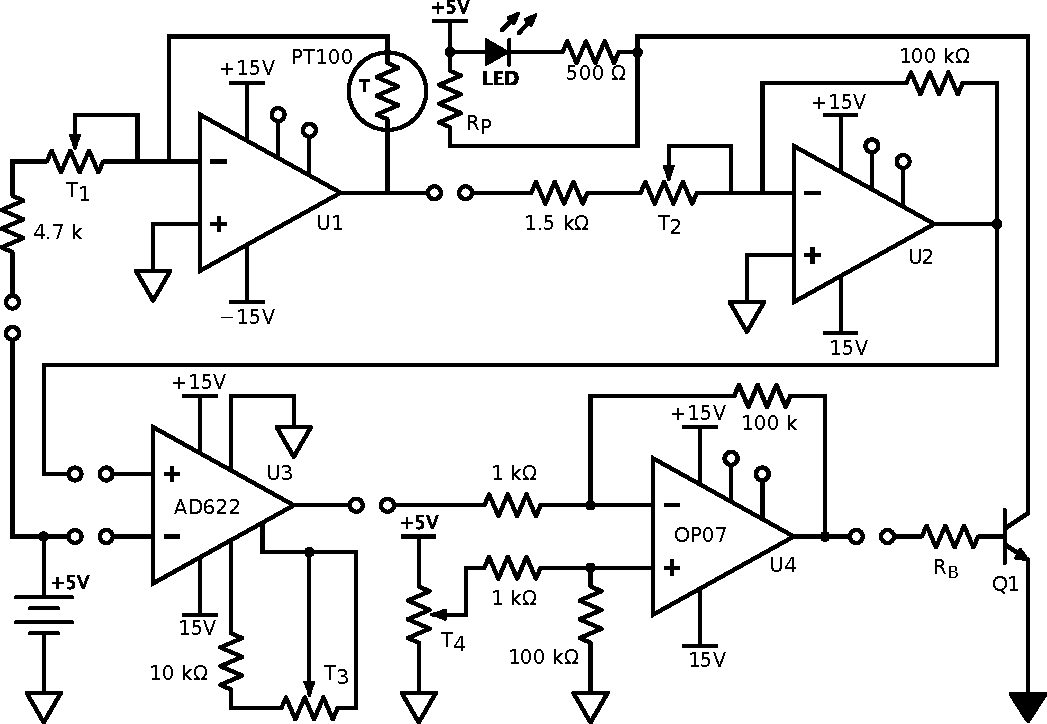
\includegraphics[width=0.78\textwidth]{../E06/latex/c2.pdf}}%.75
 \caption{Schema circuitale del sistema di controllo proporzionale della temperatura composto di un termometro elettronico e di un sistema di riscaldamento.}
 \label{gr6:proporzionale}
\end{figure}

Utilizzando la formula $G_{U3}=1+\frac{50.5k\Omega}{R_g}$ possiamo ottenere il valore di resistenza di gain: $R_g=12.038\si{\kilo\ohm}$.
Utilizzando dunque la serie tra una resistenza da $10\si{\kilo\ohm}$ e un trimmer multigiro da $10\si{\kilo\ohm}$, con l'ausilio del multimetro digitale, abbiamo tarato tale resistenza. 
Per essere sicuri che il guadagno fosse esattamente quello cercato, abbiamo fornito all'ingresso non invertente una tensione di \SI{1}{\volt} e controllato che l'uscita fosse $V_{out}=\SI{5.195}{\V}$. 

Controllati dunque tutti i moduli separatamente, abbiamo sostituito la resistenza da $100\si{\ohm}$ con la termoresistenza Pt100.
La misura di tensione all'uscita è stata $V_{out}=(2.437\pm 0.002)\si{\volt}$.
Come già detto, per ottenere la temperatura in gradi Celsius basta moltiplicare il valore di tensione per 10.
La temperatura ambiente misurata risulta dunque $T=(24.37\pm0.02)^{\circ}C$.

Abbiamo verificato il buon funzionamento del circuito raffreddando e riscaldando la termoresistenza e osservando che i valori di tensione variavano correttamente.


\subsection*{Conclusioni}

In questa esperienza abbiamo affrontato diverse problematiche, tra cui quella di progettare e costruire un circuiro composto di molte componenti.
Per fare ciò è stato necessario testare il funzionamento di singole parti dello schema complessivo per rendere più facile l'individuazione di eventuali problemi.

Nella prima parte dell'esperienza abbiamo assemblato un termometro elettronico utilizzando come sensore una termoresistenza PT100 e l'abbiamo tarato in modo tale che restituisse un valore di \SI{0}{\V} a \SI{0}{\celsius} e che scalasse di \SI{100}{\mV} ogni \SI{1}{\celsius}.

Nella seconda parte dell'esperienza invece abbiamo costruito un circuito di controllo proporzionale della temperatura.
Servendoci del primo circuito come fonte di informazione, abbiamo aggiunto due blocchi circuitali che facevano scorrere della corrente in una resistenza di potenza con il fine di riscaldare la resistenza PT100.
Inoltre questi nuovi blocchi regolavano o spegnevano l'alimentazione di tale resistenza di potenza una volta raggiunta una soglia di temperatura, decisa a priori.
In questo modo abbiamo creato un sistema termostatato ad una temperatura T da noi scelta.

\begin{figure}[ht]
 \centering
   {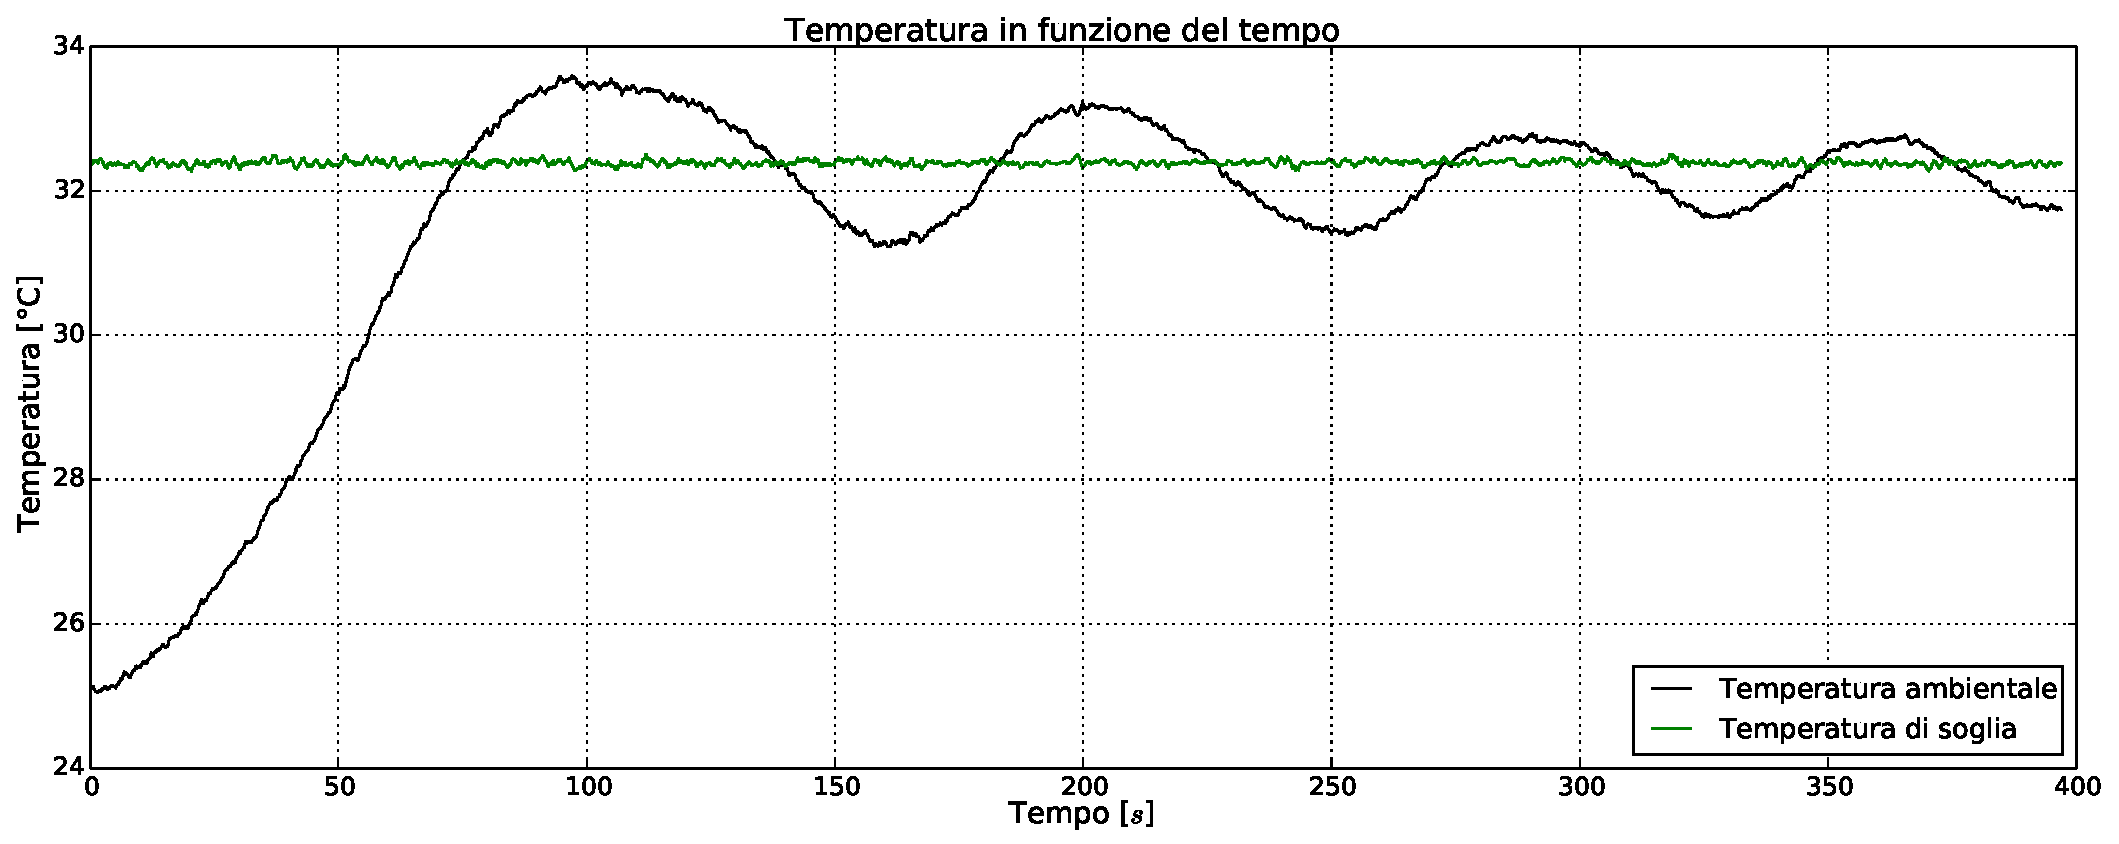
\includegraphics[width=1\textwidth]{../E06/latex/grafico.pdf}}
 \caption{Il grafico riporta la temperatura misurata dalla termoresistenza (in nero) e la temperatura di riferimento (in verde). Come si può osservare la temperatura di riferimento ha una certa instabilità data dall'instabilità della tensione all'ingresso non invertente dell'opamp nel blocco 4. L'imperferzione di tale segnale è probabilmente imputabile non all'integrato REF02, bensì a rumori ambientali.}
 \label{gr6:grafico}
\end{figure}

In Figura \ref{gr6:grafico} è rappresentato l'andamento temporale della temperatura misurata dalla termoresistenza (in nero) e della temperatura di riferimento (in verde).
Come si può notare il tempo necessario alla resistenza di potenza per aumentare la temperatura da \SI{25}{\celsius} a \SI{32.5}{\celsius} dissipando energia per effeto Joule è di circa un minuto.
Una volta raggiunta la temperatura (in realtà come abbiamo visto l'alimentazione viene prima diminuita e poi tolta completamente) il circuito esclude l'alimentazione della resistenza di potenza, ma la temperatura registrata dalla PT100 continua a salire per inerzia termica dei componenti.
Dopo poco la temperatura registrata comincia a discendere verso la temperatura ambiente, ma, una volta scesa sotto la soglia, l'alimentazione della resistenza viene riattivata alzando nuovamente la temperatura della termoresistenza.
Questi passaggi vengono ripetuti e la temperatura oscilla asintoticamente vicino alla temperatura di soglia.

Si può osservare inoltre che la temperatura di riferimento ha una certa variabilità data dall'instabilità della tensione all'ingresso non invertente dell'opamp. Tale imperferzione è probabilmente generata da rumori ambientali.
